\documentclass[11pt,letterpaper]{article}
\usepackage[lmargin=1in,rmargin=1in,bmargin=1in,tmargin=1in]{geometry}
\usepackage{style}

\setlength{\parindent}{0ex}
\usepackage{mathtools} % Overlap Symbols

\usepackage{tikzsymbols}

% -------------------
% Content
% -------------------
\begin{document}

% Title
\begin{center} {\bfseries \LARGE MATH 141 --- Comment Card Responses --- Fall 2025} \end{center}

Here are select responses to comment cards given at the end of class. When computed, the class rating (out of 10) is given. The comment (often paraphrased for clarity) is given in italics/bold with the response following the comment. The responses are labeled by class date---with the class topic given. The classes are given in reverse-chronological order for ease of access to the most recent class. You may also click any of the hyperlinks below to jump to that date.

\begin{itemize}
\item \hyperref[10-13]{10/13, Monday: Optimization}
\item \hyperref[10-08]{10/08, Wednesday: Related Rates}
\item \hyperref[10-06]{10/06, Monday: Related Rates}
\item \hyperref[10-03]{10/03, Friday: Related Rates}
\item \hyperref[10-01]{10/01, Wednesday: Implicit Differentiation}
\item \hyperref[09-29]{09/29, Monday: l'H\^{o}pital's Rule}
\item \hyperref[09-26]{09/26, Friday: l'H\^{o}pital's Rule}
\item \hyperref[09-24]{09/24, Wednesday: l'H\^{o}pital's Rule}
\item \hyperref[09-22]{09/22, Monday: Maxima, Minima, \& Inflections}
\item \hyperref[09-17]{09/17, Wednesday: Derivative Interpretations}
\item \hyperref[09-15]{09/15, Monday: Linearization}
\item \hyperref[09-12]{09/12,  Friday: Derivative Practice}
\item \hyperref[09-10]{09/10, Wednesday: Product \& Quotient Rule}
\item \hyperref[09-08]{09/08, Monday: Derivative Rules \& Chain Rule}
\item \hyperref[09-05]{09/05, Friday: Derivative Definition}
\item \hyperref[09-03]{09/03, Wednesday: Continuity}
\item \hyperref[08-29]{08/29, Friday: Limit Techniques}
\item \hyperref[08-27]{08/27, Wednesday: Limit Techniques}
\item \hyperref[08-25]{08/25, Monday: Limit Techniques}
\item \hyperref[08-22]{08/22, Friday: Limit Techniques}
\item \hyperref[08-20]{08/20, Wednesday: Graphical Limits}
\end{itemize}

% 10/13, Monday: Optimization
\newpage
\section*{10/13, Wednesday: Optimization\label{10-13}}

\begin{itemize}
\item {\bfseries\itshape Class Rating:} 8.90/10

\item {\bfseries\itshape I liked the pictures} Oh, that's terrifying as I'm a terrible artiste. 

\item {\bfseries\itshape $e - e^{ee} \cdot e \frac{e}{e} e! e^{-1} \frac{e}{e^2}$} You mean the one homework problem? It's a great exercise and I did the exact same one long, long ago!

\item {\bfseries\itshape I can't see the powers very well} I shall try to write them clearer!

\item {\bfseries\itshape Will we get the answers to the practice problems?} I do not have solutions to them written up. However, I am more than happy to discuss the solutions should you want to pop by!

\item {\bfseries\itshape It was a little hard to keep up} You can always rewatch the lecture at your own pace, pausing whenever you need!

\item {\bfseries\itshape I couldn't go that pace on a test!} You have plenty of study/practice time before the exam. I have total faith that given that time you will be able to!

\item {\bfseries\itshape Where do we plug in to find $+, -$?} If you mean for increasing/decreasing to use the 1st derivative test, you would plug those into the first derivative.

\item {\bfseries\itshape We did optimization} Yes\dots yes, we did\dots

\item {\bfseries\itshape You should make them give you more time for each class} I'm not so such we need more class time as we might benefit from reclaiming lab time. Alas, it is what it is. 

\item {\bfseries\itshape Please, do more secret endpoint/constraint problems} Oh, we shall!

\item {\bfseries\itshape Reese's?}
	\begin{figure}[H]
	\centering
	
\includegraphics[width=0.60\textwidth]{images/pieces.png}
	\end{figure}
\end{itemize}

% 10/08, Wednesday: Related Rates
\newpage
\section*{10/08, Wednesday: Related Rates\label{10-08}}

\begin{itemize}
\item {\bfseries\itshape Class Rating:} 9.00/10 [Nice when it works out so evenly!]

\item {\bfseries\itshape Thoughts on coconut pie?} I don't need to think, I \textit{know} it's gross. 

\item {\bfseries\itshape Pie slander!} Sorry not sorry. Pumpkin pie is the best average pie.
	\begin{figure}[H]
	\centering
	
\includegraphics[width=0.25\textwidth]{images/pie.jpg}
	\end{figure}

\item {\bfseries\itshape It was helpful to see how to step-by-step work out the givens} All it takes is practice!

\item {\bfseries\itshape We did related rates} \dots yes\dots yes we did\dots

\item {\bfseries\itshape I'm in CEC, this helps me model dynamic systems and calculate the [?] crucial for engineering} Oooh, I'd like to see that! Always nice to see more examples that I can maybe bring into lectures.

\item {\bfseries\itshape It makes it hard to follow along when you write less words than you say. So while I'm still writing the problem you're already started solving it} All professors do this, whether you realize it or not. We do not have time to write everything, but we do all say the important stuff. That is why developing sharp note taking skills is important. If you only ever write what the professor writes, you're doing note taking wrong!

\item {\bfseries\itshape The $xx'$ thing is confusing} You can always write $\frac{dx}{dt}$ instead of $x'$ if you would prefer. We discussed the pros/cons of $x'$ and $\frac{dx}{dt}$ in a previous lecture. Feel free to re-listen if you want it all done out again!
\end{itemize}

% 10/06, Monday: Related Rates
\newpage
\section*{10/06, Monday: Related Rates\label{10-06}}

\begin{itemize}
\item {\bfseries\itshape Class Rating:}  9.04/10

\item {\bfseries\itshape Thanks for all the extra problems!} No problemo!

\item {\bfseries\itshape Thanks!} No, thank YOU!

\item {\bfseries\itshape Why introduce the prime notation?} We have been using it all along. For instance, the derivative of $f(x)$ is $f'(x)$.

\item {\bfseries\itshape I understand this better!} That's great!

\item {\bfseries\itshape It was a confusing lecture in general} Maybe try the problems on your own later and then rewatch the video comparing your solution to what we did. Sometimes, trying it for yourself first helps makes things clearer. 

\item {\bfseries\itshape There's a Wegmans opening in Charlotte next year} I'd drive that far for it.
\end{itemize}

% 10/03, Friday: Related Rates
\newpage
\section*{10/03, Friday: Related Rates\label{10-03}}

\begin{itemize}
\item {\bfseries\itshape Class Rating:} 8.53

\item {\bfseries\itshape How many different problems are there?} Dozens upon dozens upon dozens. However, once you get to the third step of our procedure, you will notice that the same equations are written down again and again. So, in some sense, there are very few problems---likely 5--8. 

\item {\bfseries\itshape I understand how to solve these!} Isn't that feeling of `I got this' great?

\item {\bfseries\itshape That was well paced!} Are they all not?

\item {\bfseries\itshape I always think related rates are fun at the beginning but we'll see if that lasts} They are fun at the beginning. They are fun in the middle. And they are especially fun at the end. 

\item {\bfseries\itshape I caught the Pretty Woman reference. That was fun!} You mean what I said or that I was a pretty woman?

\item {\bfseries\itshape I was a little confused but I'll just email my question} I'll be waiting for it!

\item {\bfseries\itshape You did a great job with related rates!} Great? Not amazing or perfect?

\item {\bfseries\itshape What is the average wing beat of an English swallow? (Prove it with Math)} Don't you ean the airspeed of an unladen swallow? 

\item {\bfseries\itshape Squids control everything!} 
	\begin{figure}[H]
	\centering
	
\includegraphics[width=0.40\textwidth]{images/squid.jpg}
	\end{figure}

\item {\bfseries\itshape Not seeing the logic yet. Need more examples} And you shall have them! Also\dots homework.

\item {\bfseries\itshape It's cold in here} \href{https://www.youtube.com/watch?v=xm3YgoEiEDc\&list=RDxm3YgoEiEDc}{It's like that song!}

\item {\bfseries\itshape Have you watched Macabre (1958)?} You mean Macbeth (1971)? Yes. Otherwise, no.

\item {\bfseries\itshape Do you consider yourself more of a nerd, dork, or geek?} I prefer to think of myself more as the centaur goddess Diaphena hunting a stag\dots or whatever a potato feels like after it starts growing eyes.

\item {\bfseries\itshape To be clear, all 3 Human Centipede movies are abominations} Not the first. But the third is indeed the worst movie ever made. 

\item {\bfseries\itshape Why don't you like RedDead?} One word: pacing. More words: for instance, he controls like a watermelon attached to the top of a broom and runs at a Stephen Hawking off-roading pace. 

\item {\bfseries\itshape Based game recommendations} I don't know any. Is that a shooting game subgenre? 

\item {\bfseries\itshape Did you ever play Binding of Isaac?} Nope.
\end{itemize}

% 10/01, Wednesday: Implicit Differentiation
\newpage
\section*{10/01, Wednesday: Implicit Differentiation\label{10-01}}

\begin{itemize}
\item {\bfseries\itshape Class Rating:} 9.09/10

\item {\bfseries\itshape  What do you mean independent versus dependent?} This is probably best addressed with an example. If $y= x^3$, then $x$ depends on $x$, i.e. is dependent. If $x^2 + y^2= 1$, then $y$ depends on $x$ too---given an $x$, $y$ cannot be just anything to make the left side be 1, so $y$ depends on $x$. However, given a point $(x, y)$, $y$ is independent from $x$. You can choose their values independently. If $y= 3t - 4$, then $x, y$ are independent. Yes, $y$ depends on something else but not $x$. 

\item {\bfseries\itshape When do we use implicit differentiation?} Any time you want something that requires it, e.g. $\frac{dy}{dx}$, but $y$ has only an implicit relationship with $x$, e.g. $x^2 + y^2= 1$. 

\item {\bfseries\itshape This was a little fast} Sorry. Maybe a rewatch of the lecture video where you pause as needed to think things through?

\item {\bfseries\itshape More practice sessions!} That is what recitation is for!

\item {\bfseries\itshape I thought it was all helpful!} Glad you found it helpful!

\item {\bfseries\itshape I actually got everything today\dots :D} Victory screech!
	\begin{figure}[H]
	\centering
	
\includegraphics[width=0.25\textwidth]{images/screech.jpeg}
	\end{figure}

\item {\bfseries\itshape You make me feel stupid when I ask questions} I am sorry that you felt that way during class. It's always perfectly fine to ask questions---you're learning! Know despite what my friends have termed by `resting bitch face', I am never judging your questions, especially when I make faces. It's very hard to hear folks and also make sense of what people are trying to ask. Math is like a foreign language that you guys are learning but that I speak fluently. It's understandable that you won't use the correct words or phrase things like a mathematician would or not articulate things `naturally' but then it really throws me off balance. So, it's like when a non-native speaker asks, ``If you bubble cook the white liquid, does cheese it make or is that differently?'' [Do you boil milk to make cheese or is some other process?] I have to hear it, make sense of it, and then come up with an answer that will also make sense to everyone---all in the span of a second or two---and it can really throw me off sometimes. But never stop asking questions! 

\item {\bfseries\itshape Watch the movie Threads if you haven't already} You mean the 1984 film?

\item {\bfseries\itshape Thoughts on Tusk, the movie?} Never heard of it. But pulling it up, I'm surprised because it has Justin Long and I love Justin Long\dots then again it has Haley Joel Osmet and seeing him nowadays just makes me sad. By the way, Justin Long's best moment on film is his introduction in Zack and Miri Make a Porno.

\item {\bfseries\itshape Favorite check-in quote by far} I mean Hocus Pocus is an S-tier Disney Movie. Bette Midler is a treasure---great music. Did you know she was from Hawaii before it was even a state? Also, did you know she got her start singing in a gay bathhouse in NYC?
\end{itemize}

% 09/29, Monday: l'Hopital's Rule
\newpage
\section*{09/29, Monday: l'H\^{o}pital's Rule\label{09-29}}

\begin{itemize}
\item {\bfseries\itshape Class Rating:} 8.94/10

\item {\bfseries\itshape Does $\infty^0$ have similar rules to $0^\infty$:} Not at all! Remember, l'H\^{o}pital's can only be applied to $\frac{0}{0}$ or $\frac{\infty}{\infty}$. Yes, we ultimately also use it in the cases of $\infty - \infty$, $0 \cdot \infty$, $1^\infty$, $0^0$, and $\infty^0$, but these are still all indeterminant forms. That is, we only ever use l'H\^{o}pital's rule with indeterminant forms. But $0^\infty$ is not an indeterminant form! So, you will never use l'H\^{o}pital's with this.

\item {\bfseries\itshape It was nice you went around to help} Always happy to help! Remember, you have lots of help available to you at USC!

\item {\bfseries\itshape Please, keep explaining how ``fat'' numerators push into denominators. Helps a lot} Sarcasm? In any case, I don't believe I said `fat.' I believe I said `full bodied.'

\item {\bfseries\itshape I'm so lost. Math is hard} It's understandable to be lost. But what you do not want is to stay lost. So, seek help! You have lots of help available to you at USC! Learning to drop the `shame' with being lost/confused is definitely a great thing to help you go as far as possible in college. There's never a shame in asking for help.

\item {\bfseries\itshape How do you know if its $\infty^0$ or $\frac{\infty}{\infty}$?} We always try plugging in the limiting value first. If you do and you get one of those forms, then it is one of those types of l'H\^{o}pital's.

\item {\bfseries\itshape Can you go over how to set the limit up in order to use l'H\^{o}pital's?} Yes/No? We do a lot of this, but there's no series of steps that will always work as it depends on the problem. However, I did give rules of thumb for each case. [See the Learning Outcomes document.]

\item {\bfseries\itshape When does l'H\^opital's not work?} You will notice it when the problem becomes more difficult with each application of l'H\^{o}pital's or when the problem `loops' back to the original limit. 

\item {\bfseries\itshape I hate derivatives} Not everything is everyone's cup of tea. However, it is essential to be very good at them! They will not go away for the rest of the semester---and likely the rest of your math courses. Moreover, usually taking the derivative is only a small part of the problem. So, being good and fast at them allows you to focus on the `meat' of the problem.

\item {\bfseries\itshape I understand this better now} That's great!

\item {\bfseries\itshape Rate South Park out of 10} Across all seasons? 8.6/10

\item {\bfseries\itshape [Hollow knight drawing]} Nice!

\item {\bfseries\itshape Call the set of primes a royal flush} I'm not sure that I get it?

\item {\bfseries\itshape Is the ``cool cool cool'' you do a Brooklyn 99 reference?} No, the show that did it first.
	\begin{figure}[H]
	\centering
	
\includegraphics[width=0.35\textwidth]{images/coolcoolcool.png}
	\end{figure}
\end{itemize}

% 09/26, Friday: l'Hopital's Rule
\newpage
\section*{09/26, Friday: l'H\^{o}pital's Rule\label{09-26}}

\begin{itemize}
\item {\bfseries\itshape Class Rating:} 8.44/10 

\item {\bfseries\itshape I liked the examples} There are lots more in the homework!

\item {\bfseries\itshape Examples} There are \textit{lots} of really great examples with solutions in the `External Resource' folder in Blackboard. 

\item {\bfseries\itshape Great lecture I just got lost} Then feel free to ask questions or stop by for help!

\item {\bfseries\itshape I am not sure what case is which} This might take some study and practice. Maybe try making flashcards of what you do for each case of l'H\^{o}pital's Rule?

\item {\bfseries\itshape I need help} Then reach out for help! There are \textit{lots} of options for you: myself, the TA, the SI, the other SI sessions, the Math Lab, tutoring, etc.

\item {\bfseries\itshape Yotai} Do you mean Y$\overline{\text{o}}$ei, as in Ghost of Y$\overline{\text{o}}$ei? Yes, I am very excited for it this week. Ghost of Tsushima is a top 5 game for me. 

\item {\bfseries\itshape Thanks for being an efficient teacher and part time comedian} Obviously, you haven't seen me at my night job where I am definitely a full-time comedian. 

\item {\bfseries\itshape ``This is where you push past your limits kid.'' --Yami} Such a great show\dots at first. Then it just ruined its potential and became so mid.  
\end{itemize}

% 09/24, Wednesday: l'Hopital's Rule
\newpage
\section*{09/24, Wednesday: l'H\^{o}pital's Rule\label{09-24}}

\begin{itemize}
\item {\bfseries\itshape Class Rating:} 9.08/10

\item {\bfseries\itshape  Will l'H\^{o}pital's be on the Gateway?} Nope! Gateway II is only derivatives. 

\item {\bfseries\itshape How does quotient rule apply to l'H\^{o}pital's rule?} Nothing! It has nothing to with it---so be sure to keep them very separate in your head!

\item {\bfseries\itshape The algebra involved in the examples is hard} Practice makes perfect! Remember, you can always get help to review these topics!

\item {\bfseries\itshape Your shirt is funny} Nerd shirts are the best shirts.

\item {\bfseries\itshape When do you use l'H\^{o}pital's rule versus another technique?} You can always use it whenever it applies. But when is it the way to go versus old techniques? That really depends on the problem. I cannot really give generic rules that will hold all the time. It's about experience until you get a `feel' for it.

\item {\bfseries\itshape That was a good explanation of l'H\^{o}pital's} Thanks!

\item {\bfseries\itshape Great jokes!} Nice that I'm appreciated for being funny rather than just looking funny.

\item {\bfseries\itshape I just need to come by office hours} Stop on by! 

\item {\bfseries\itshape The jokes slapped} Danke!

\item {\bfseries\itshape Did I do well on the exam?} I do not know anonymous commenter! 

\item {\bfseries\itshape Why do people love this rule?} Probably because those that saw Calc before typically remember this---for whatever reason---and it feels good to really remember/be able to use something. Otherwise, I assume because it's `direct'---you can just apply it. So, there's less clever thought/work compared to some of the other limit techniques.

\item {\bfseries\itshape I think the accent in l'H\^{o}pital's rule is called a circumflex} I looked it up. Indeed, you are correct. Apparently, it's a change in French spelling from what used to be `os', hence the `hospital'. You also see this in anc\^etre (ancestor), h\^otel (hostel), r\^otir (roast), c\^ote (rib/coast/slope), p\^ate (paste), etc.

\item {\bfseries\itshape How much is considered a good bribe to you? [I am a broke college student]} Considering it would end my career, enough to finish off my career. So, about \$3,000,000--\$5,000,000.

\item {\bfseries\itshape What function is always runny? A \underline{sinus}-oidal function} Boo
	\begin{figure}[H]
	\centering
	
\includegraphics[width=0.4\textwidth]{images/boo.png}
	\end{figure}
\end{itemize}

% 09/22, Monday: Maxima, Minima, \& Inflections
\newpage
\section*{09/22, Monday: Maxima, Minima, \& Inflections\label{09-22}}

\begin{itemize}
\item {\bfseries\itshape Class Rating:} 8.67/10

\item {\bfseries\itshape Is the test multiple choice or open ended?} I never reveal what an exam will look like. However, it is unlikely to drift super far from the last few exams.

\item {\bfseries\itshape Is concavity going to be on the exam?} Exam 1? No. Exam 2? It is a perfectly valid exam topic. 

\item {\bfseries\itshape It was hard to see the board} Maybe beat someone to one of those coveted front row seats!

\item {\bfseries\itshape I just need more time to understand} That's understandable!  Study, practice, and always ask for help if you need it!

\item {\bfseries\itshape It's cold in here} I love the cold!

\item {\bfseries\itshape I need caffeine} Me too. Always

\item {\bfseries\itshape Learning that concave down is also called convex was genuinely helpful. It clarified a point of confusion on that I'd struggled} \dots not to ruin a moment, but it's concave up that's convex. Concave down is concave.

\item {\bfseries\itshape Waste of paper. Plz consider online survey (QR)} Absolutely not. I have tried this in the past. Students do not do it when it's a QR code---not that they always do it in these form. An online format is more rigid. But worst of all, nearly all digital forms allow (or at least can) tracking of who submits what. Even if I turn that off, students will always wonder if I'm tracking the comments, which greatly defeats the purpose. Because I cut 10 to a page, a single ream of paper sets me for over a semester for all my classes comment cards. It is absolutely worth it.

\item {\bfseries\itshape Miss the pre-printed notes} Most don't. It really is like 50-50 or so on whether folks like them or not.

\item {\bfseries\itshape I am gonna bomb this exam \#doomsday} Why the gloom and doom? You have plenty of time to study, practice, and prepare to make sure that's not the case! Ask for help if you need it!

\item {\bfseries\itshape You da man} I guess?

\item {\bfseries\itshape Thanks for breaking it down!} Always try at least!

\item {\bfseries\itshape Cheeseburger} God, I love burgers.

\item {\bfseries\itshape Is German your favorite language?} Yup!
\end{itemize}

% 09/17, Wednesday: Derivative Interpretations
\newpage
\section*{09/17, Wednesday: Derivative Interpretations\label{09-17}}

\begin{itemize}
\item {\bfseries\itshape Class Rating:} 9.17/10

\item {\bfseries\itshape I get confused with what to plug into what} That comes with practice. But what can really help is really knowing what is in the word clouds I gave you. Because if you know those well, as you plug in, you can think what the `thing' you are plugging into gives you and then consider is that what you want?

\item {\bfseries\itshape What is a global versus a local max/min?} A global max/min is the largest possible/smallest possible output, respectively, for a function. Whereas a local max/min is simply one larger/smaller, respectively, than the outputs `near' its corresponding $x$-value. A function need not have either a global max or a global min.

\item {\bfseries\itshape Nice new haircut. Looking spiffy twin} Thanks! I cut my own hair.

\item {\bfseries\itshape I liked the examples} Glad you found it helpful!

\item {\bfseries\itshape I understood this!} Isn't it a great feeling! Always seek that feeling out!

\item {\bfseries\itshape The pace was nice!} Glad you found it good for you!

\item {\bfseries\itshape 5 Guys Burgers} Truly, an S-tier fast food burger. 

\item {\bfseries\itshape Good job Caleb} Danke!

\item {\bfseries\itshape What is the point of the second derivative test?} As mathematicians, we are always trying to understand things as thoroughly and deeply as possible. So, knowing/having yet another test is important---even if it isn't as helpful in the 1-dimensional case. However, unlike the first derivative test, the second one is actually the one that generalizes to more than one variable, whereas the first one becomes useless. 

\item {\bfseries\itshape Favorite food?} Sushi. Always

\item {\bfseries\itshape Mondays are dumb} So are any non-weekend days.

\item {\bfseries\itshape Do professors look at their RateMyProfessors?} The older the professor, the less likely they are to really ever look at it. The younger generation might, but only rarely. I, myself, might only look at it every 6~months or so. Remember, the only people that go on it to leave a review are the really disgruntled or the big fans---skewing the results. Hard to give a website that used to have students rate their professors hotness much weight\dots and I am not spiced that I didn't get a hot tamale. Not. At. All. A professors actual course evaluation numbers likely greatly differ from RateMyProfessors. My actual numbers typically put me (if forced out of 5) between a 3.8 and 4.8, depending on the course, section, and semester. It varies. 

\item {\bfseries\itshape ?`Hablas espa\~nol?} S\'i, entiendo espa\~nol, pero hace mucho tiempo desde que lo us\'e. Si tuviera tiempo, me gustar\'ia repasarlo m\'as. 
\end{itemize}

% 09/15, Friday: Derivative Practice
\newpage
\section*{09/15, Monday: Linearization\label{09-15}}

\begin{itemize}
\item {\bfseries\itshape Class Rating:} 8.49/10

\item {\bfseries\itshape What's normally the pass rates for exams?} It depends on the semester and the exam. But for the first exam, the pass rate is typically 49.86\%, but not normally distributed. 

\item {\bfseries\itshape Please show ways/methods to memorize the derivatives of arc functions} I do not know of any tricks for this. Sometimes, you just gotta put in the work---no tricks. There's also only 6 of them, so it should be quick.

\item {\bfseries\itshape Just need more time with this} That's fine and expected for some topics! Some things take longer than others to `get'. All that matters is that you put in the work to make it happin', captin'.

\item {\bfseries\itshape Are you required to simplify fractions like we had $\frac{620}{320}$. Do we need to reduce to $\frac{62}{32}$?} We had $\frac{621}{320}$, not $\frac{620}{320}$, which is why we did not reduce. Notice that $\frac{621}{320}$ does not reduce. Otherwise, we would have reduced---as one should. However, the point of this topic is typically to find decimal values. So, normally we would convert to decimals. It's just that $\frac{1}{32}$ was not simple to do that with (unless you remember $\frac{1}{8}= 0.125$), so we just left things as a fraction. 

\item {\bfseries\itshape What do you mean $\sin \theta \approx \theta$?} Let $f(\theta)= \sin \theta$. Let's find the linearization of $f(\theta)$ at $\theta= 0$. We have $f(0)= \sin(0)= 0$. We also have $f'(\theta)= \cos \theta$ so $f'(0)= \cos(0)= 1$. Therefore, the linearization of $f(\theta)$ is $\ell_0(\theta)= f(0) + f'(0) (\theta - 0)= 0 + 1(\theta - 0)= \theta$. We know that $f(\theta) \approx \ell(\theta)$ for $\theta \approx 0$. But then for `small' angles $\theta$, we have $\sin \theta \approx \ell_0(\theta)= \theta$, i.e. $\sin \theta \approx \theta$ when $\theta$ is `small' (close to 0). This is known as the small angle approximation for $\sin \theta$.

\item {\bfseries\itshape How do I know when to stop? How do I find the percent error?} I'm not sure what you mean by the first question. But for the second, it is $\left| \frac{\text{predicted} - \text{actual}}{\text{actual}} \cdot 100 \right|$. For instance, if $f(3.1)= 16.434$ but the linearization yielded $\ell(3.1)= 15.889$, then the percent error is\dots
	\[
	\left| \dfrac{15.889 - 16.434}{16.434} \cdot 100 \right|= \left| \dfrac{-0.545}{16.434} \cdot 100 \right|= |-0.033163 \cdot 100| \approx 3.32\%
	\]
So, the error in the approximation was 3.32\%. 

\item {\bfseries\itshape The examples were great} Thanks! Glad you liked them. There are even more in the homework. \Winkey

\item {\bfseries\itshape The beginning explanation with the graph was a little difficult to follow} Oof. I tried my best. But remember, you can always watch the lecture again to try and catch the opening. Sometimes, it's easier the second time because you have a better idea of where things are going.

\item {\bfseries\itshape Need more practice} There's plenty on the homework\dots \Winkey

\item {\bfseries\itshape Brain not braining} Oof. It be like that sometimes.

\item {\bfseries\itshape This lesson was confusing} Maybe try a rewatch? Sometimes, you just need to try it again---likely easier the second time because you know where things are going.

\item {\bfseries\itshape Everything was relatively/somewhat easy to understand} Glad you thought so! You can see how much it made sense by trying the homework!

\item {\bfseries\itshape Please rewrite the formula you're plugging in when solving examples} I did for the first example, I just did less so for the second.

\item {\bfseries\itshape The writing was a bit fast and small} Sorry. I forget/fail sometimes.

\item {\bfseries\itshape USC or Syracuse, which is better?} Why does one have to be better than the other?

\item {\bfseries\itshape Can you zoom in?} I shall try! Always give a shoutout if you can't read something.

\item {\bfseries\itshape Could you slow down?} When it comes to lecture topics, I can try. But I really already try and pace myself to go as slowly as possible while still covering exactly what we need to cover. The time is rather tight (per lecture and across the semester). Remember, you can always watch it back and pause! It's often easier the second time because you know where things are going and you only really have to focus on the things you did not understand the first time. 

\item {\bfseries\itshape Wish we got more practice} There's plenty on the homework \Winkey

\item {\bfseries\itshape What do you mean by `close'?} We cannot make that precise---not in this course. We shall just `eyeball' or assume `close' is `close'. How `close' $x$ needs to be to $a$ depends on the function and the $a$-value. What we do know is that the `closer' $x$ is to $a$, the more accurate the linearization will be in approximating $f(x)$.

\item {\bfseries\itshape What is your opinion on cheese?} You mean rotten milk? Who do I look like, Charlie?
	\begin{figure}[H]
	\centering
	
\includegraphics[width=0.35\textwidth]{images/cheese.jpg}
	\end{figure}
\end{itemize}

% 09/12, Friday: Derivative Practice
\newpage
\section*{09/12, Friday: Derivative Practice\label{09-12}}

\begin{itemize}
\item {\bfseries\itshape Class Rating:} 9.21/10
\item {\bfseries\itshape Please go over when using product rule what you copy after deriving} I usually do, at least to me, by saying what it is I am doing. But I totally understand if it can be hard to follow if you're having some trouble with derivatives. Remember, always feel free to stop by any of us (me, TA, or SI) for help! The product rule is a `one at a time' rule. So, you do the derivative of \textit{one} of the things in the product, and the others are copied. You continue this one at a time until you have done the derivative of each function in the product once---remembering to add in between them. For example, suppose we have $f(x)= e^{-x} \cos(5x) \sec^{-1} x$, then (just choosing to do the derivative left to right) $f'(x)$ would be\dots
	\[
	\underbrace{(e^{-x} \cdot -1)}_{\tfrac{d}{dx} e^{-x}} \cdot \underbrace{\cos(5x) \sec^{-1} x}_{_{\text{copied part}}} + \underbrace{(-\sin(5x) \cdot 5)}_{\tfrac{d}{dx} \cos(5x)} \cdot \underbrace{e^{-x} \sec^{-1} x}_{_{\text{copied part}}} + \underbrace{\left( \dfrac{1}{|x| \sqrt{x^2 - 1}} \right)}_{\tfrac{d}{dx} \sec^{-1} x} \cdot \underbrace{e^{-x} \cos(5x)}_{\text{copied part}}
	\]

\item {\bfseries\itshape The two exams you posted online, are these a good indication of what is on the exam?} You are in no way guaranteed that the exams will look exactly like that or even close to that. They are a good indication of what types of questions you might see if that topic appears on the exam. They are also a good indication of the `balance' of the material on the exam. Of course, the material is the material and it's what we want you to learn. So, you will notice patterns, focus, and types of questions that are typically on it. No matter what, being able to do them and do well on them is an indication of your level of preparedness for the exam. 

\item {\bfseries\itshape You seemed to be reiterating the \underline{if} these were on the test thing. Are some of these on the test?} I do not teach to tests because that is not learning. I want ya'll to learn the material well enough that you could do well on any test in any class---indeed, especially your future classes. The `ifs' were to keep you aware of exam expectations and pacing. 

\item {\bfseries\itshape Do we copy for every derivative?} Yes! Every derivative rule includes some pieces that simply need to be copied at each stage. 

\item {\bfseries\itshape Will there be any real exam reviews on Blackboard? The ones currently posted are Rick-Rolls} I think you are looking at this semesters exams and solutions, which cannot be released before they are given! However, the old semester exams and solutions are posted but not on Blackboard. These are on my webpage, which is linked on Blackboard. I link to each old class on Blackboard. I also sent an email giving a suggested study outline for the exam. 

\item {\bfseries\itshape Is partial credit given on the exams?} Of course! Not necessarily on every question. But overall, there is partial credit to be earned. 

\item {\bfseries\itshape We do we have to simplify everything on Pearson when we are not supposed to?} You don't. As I said in class, Pearson is not checking for simplification unless specified. So, entering $x \cos x \cdot 2x$ as your answer would be accepted as correct as if you had entered $2x^2 \cos x$. If you are marked wrong, that is because you are incorrect or typed your answer incorrectly. 

\item {\bfseries\itshape When changing a function from a quotient rule to a quotient [sic] rule, I do; $\frac{d}{dx} \left( \frac{f}{g} \right) \to \frac{d}{dx} \left(f \cdot g^{-1} \right)$? Then follow normal prod rule?} Indeed! For example,
	\[
	\dfrac{d}{dx} \left( \dfrac{\sin x}{5x + 1} \right)= \dfrac{d}{dx} \sin x (5x + 1)^{-1}= \cos x \cdot (5x + 1)^{-1} + \left( -1(5x + 1)^{-1} \cdot 5 \right) \cdot \cos x
	\]

\item {\bfseries\itshape Is there a better way to identify what we use other than repetition (math in general)} There is a rule for each derivative rule. For instance, chain rule you can use all the time---or when you have a composition. Product rule is for derivatives of products and quotient rule is for derivatives of quotients. Of course, I think doing enough problems until you get a `feel' for things is really the best way of doing things. Eventually, you won't even think about the rules. 

\item {\bfseries\itshape Do you write down and remember each check-in quote or do you just search for a random one the day you assign the check-in?} I have a massive collection of TV/movie quotes I have collected myself. I select from these. So, yes, each quote is `hand selected.' 

\item {\bfseries\itshape Thanks for study email guide} No problem! I hope that it works for you!

\item {\bfseries\itshape You make me like math} Careful now! Next thing you know, you'll love math. Then you'll be doing it all night long. You might even make a career of it. 

\item {\bfseries\itshape It was nice to be able to see my common mistakes} Great! It's like Mrs. Frizzle said, ``Take chances, make mistakes, get messy!'' Remember, you can always stop by myself, the TA, or the SI for them to comment on work to see if it is right or wrong and the write-up of the solution. 

\item {\bfseries\itshape Slow down please, I am barely holding on} I try to go as slow as we can in class. It might be the case that you need some temporary extra support! There's absolutely no problem with that. Remember, there's a lot of resources available to you and lots of people there to help! I've listed out many in this document and there are lots linked in Blackboard as well as mentioned in the syllabus. 

\item {\bfseries\itshape Can we have more days where we do exam like questions like this?} There are exam review days built-in, but for the other exams. You should have another review day in recitation though!

\item {\bfseries\itshape I really like having a few days to practice} There's even more practice available in the homework \Winkey

\item {\bfseries\itshape I liked our examples/practice based class, I would like to do limits practice and/or definition of a derivative practice} You should have had one of these in recitation! 

\item {\bfseries\itshape Can we do hard exam level limit problems with this format?} You should have had a day or two in recitation for exactly this thing! But, in any case, there will be exam review in recitation coming up. 

\item {\bfseries\itshape Super helpful to have practice that mirrors the test! Thank you} I was more mentioning for pacing, but they were exam worthy problems.

\item {\bfseries\itshape Doing a great job man} Thanks! But if you looked at my life more carefully, a more apt description would be `child'. 

\item {\bfseries\itshape You da mom} \dots I don't know how to feel about this.

\item {\bfseries\itshape Would love to spark a $\star\star\star\star\star$ and do some calc $\star\star\star\star$} Inappropriate. 

\item {\bfseries\itshape I think the Jim Carrey movie you were thinking of is Liar Liar} No, it was `I Love You Phillip Morris'.

\item {\bfseries\itshape I appreciate your explanations \& style of derivatives} Thanks! Hope they work for you. 

\item {\bfseries\itshape The practice was great} The key to doing well in all the Calculus/Differential Equations courses is lots of practice. 

\item {\bfseries\itshape 1 gorilla vs 50 men (no weapons) who wins? Fear is not a factor} Haven't you seen `We Crashed'? The person that wins is the one with all the money. 
\end{itemize}

% 09/10, Wednesday: Product & Quotient Rule
\newpage
\section*{09/10, Wednesday: Product \& Quotient Rule\label{09-10}}

\begin{itemize}
\item {\bfseries\itshape Class Rating:} 9.25/10

\item {\bfseries\itshape What are some of the applications of derivatives?} Don't worry, we will get to them! Although, we will only begin to scratch the surface this semester. I am always more than happy to discuss more of them outside of class. 

\item {\bfseries\itshape I don't like product rule having embedded chain rules} Just you wait, we'll have even more rules happening all at once! But don't worry, we build there slowly so you will have the skills by the time we get to those. Luckily, the derivative we do `in a vacuum' are often harder than the ones we work with in practice.

\item {\bfseries\itshape It's hard for me to tell when to use the chain rule} You can always use the chain rule! For example, if I wanted the derivative of $\sin x$, you might think, ``That's just $\cos x$.'' Correct! But I can even think of that as coming from the chain rule: the derivative of $\sin$ is $\cos$, so we have $\cos x$ but then I have to multiply by the derivative of the `next layer down', which is $x$. The derivative of $x$ is 1. So, the derivative should be $\sin x \cdot 1= \sin x$. There is never any harm in applying it so long as you do correct things! Over time, you will become more confident in when you need it and when you don't. 

\item {\bfseries\itshape Thanks for making this simple!} Simple, maybe. Easy, no!

\item {\bfseries\itshape Do you have to solve anything for quotient rule?} I'm not sure what you mean by solve for anything. It's not an equation. But there are things that you need to find. 

\item {\bfseries\itshape Since I'm squared, I'll be fair} Oh, that like has a rhythm to it! 

\item {\bfseries\itshape Giga chad} For whatever reason, whenever I hear this all I think of is\dots
	\begin{figure}[H]
	\centering
	
\includegraphics[width=0.45\textwidth]{images/skin.jpg}
	\end{figure}

\item {\bfseries\itshape Alt+$\mathrlap{\text{\textbackslash}}{\mathcal{U}}$Fu=\$} \dots what???

\item {\bfseries\itshape Genuinely thank you for the simple versions of product/chain/quotient rules!} That's what I do.

\item {\bfseries\itshape \dots Math just sucks} Oof. Sorry you feel that way. It's not fun to be stuck in something that you don't like or struggle with it. But find the perseverance, you will get through! We're all here to help you make that happen. 

\newpage

\item {\bfseries\itshape Thanks!}
	\begin{figure}[H]
	\centering
	
\includegraphics[width=0.40\textwidth]{images/citizen.jpeg}
	\end{figure}

\item {\bfseries\itshape Hidy lowdy, lowdy what?} Exactly. Not my recommendation for remembering quotient rule\dots unless it works for you. 

\item {\bfseries\itshape I was genuinely really confused. I will attend your office hours} No problem at all! You can always feel free to stop by and ask questions or ask for clarification. It's fine to need some more time or need some more help. You can also attend SI sessions, visit the Math Lab, attend tutoring, or see your TA!

\item {\bfseries\itshape Is there an SI for this class?} There is an SI for each class. Which SI depends on your section. However, you can attend SI sessions for \textit{any} section. The schedule for the SI sessions can be found here: \url{https://sc.edu/about/offices\_and\_divisions/student\_success\_center/study-smart/supplemental-instruction/si-schedule/index.php}

\item {\bfseries\itshape Your weird ass quotient rule thing was helpful} Glad you maybe found it helpful. I won't say it's good. I will say it's a thing.

 \item {\bfseries\itshape You gave two different formulas to solve the same problem} I'm not sure what you mean by this? All the methods we looked at are all the same---there's only one identity per method. How I do derivatives is not a different formula so much as it's a different perspective. 
 
 \item {\bfseries\itshape I wish I knew we would cover this before I did the HW\dots} We will always cover everything that you need for the homework! You can always check the course schedule to see when we will finish topics to then have everything that you need for the homework. 

\item {\bfseries\itshape you pookie} No, I'm Caleb.
	\begin{figure}[H]
	\centering
	
\includegraphics[width=0.40\textwidth]{images/patrick.png}
	\end{figure}

\item {\bfseries\itshape lo di high, high di lo} Or is it high di lo, lo di high? That's my problem. They sound the same!

\item {\bfseries\itshape Thanks for the quotient rule}. You're welcome but\dots like \dots I had to teach it.

\item {\bfseries\itshape Rules + stuff} I love rules. It's where I get my rules\dots and most of my stuff.
	\begin{figure}[H]
	\centering
	
\includegraphics[width=0.40\textwidth]{images/ron.png}
	\end{figure}

\item {\bfseries\itshape Hey} Hey is for horses. Grass is cheaper, unless you're smoking it.

\item {\bfseries\itshape Very silly}
	\begin{figure}[H]
	\centering
	
\includegraphics[width=0.30\textwidth]{images/goose.jpg}
	\end{figure}

\item {\bfseries\itshape Why do you wear glasses, you seem like a bifocal guy} I'm not sure you can tell that from the glasses? 
\end{itemize}

% 09/08, Monday: Derivative Rules \& Chain Rule
\newpage
\section*{09/08, Monday: Derivative Rules \& Chain Rule\label{09-08}}

\begin{itemize}
\item {\bfseries\itshape Class Rating:} 9.14/10

\item {\bfseries\itshape Is email the best method of contact?} Just speaking to me is probably best, but otherwise email is best. Email over Blackboard for sure too. 

\item {\bfseries\itshape Could you help us understand the definition and functions of derivatives more?} I would love to be able to do more lectures on it, but we have to move on. However, I'm always happy to talk about it more or work on problems with you during/outside office hours! I am sure your TA will bring it up. You can also visit their office hours, or the SI sessions, or visit the Math Lab or sign up for tutoring! There's lots of resources to help you!

\item {\bfseries\itshape What are other examples of continuous functions that are not differentiable?} I think the easiest example to construct that is everywhere continuous but nowhere differentiable is the Blancmange function, \url{https://en.wikipedia.org/wiki/Blancmange\_curve}

\item {\bfseries\itshape Will the exam study guide be posted to Blackboard?} I will be posting an exam study outline.

\item {\bfseries\itshape I am struggling with limits on the homework, especially evaluating what the limit is from left or right side. Which video/lectures do you recommend going over?} In the `External Resource' folder on Blackboard there is a whole folder full of them!

\item {\bfseries\itshape Life saver with the box method. Thank you!} Glad you liked it. Just be sure to practice so you can use it on your own!

\item {\bfseries\itshape I don't like the chain rule} Why?! It's bread and butter. And both bread and butter are awesome!

\item {\bfseries\itshape It was a little fast paced} Sorry. We will get a problem day to just practice them!

\item {\bfseries\itshape I liked your chain rule method} I think boxes really are the way to go!

\item {\bfseries\itshape I liked the box method.} Thanks! Just be sure to practice it!

\item {\bfseries\itshape Box method was great!} Thanks! Now try the homework problems to make sure it all clicks on your own!

\item {\bfseries\itshape Thank you for being a good calc teacher :P } Good?! Not great?!

\item {\bfseries\itshape The Shrek Rule was helpful} Again, all life lessons come from Shrek. 
	\begin{figure}[H]
	\centering
	
\includegraphics[width=0.30\textwidth]{images/onion.jpg}
	\end{figure}

\item {\bfseries\itshape F**k da chain rule} Love da chain rule. It's off the chain.

\item {\bfseries\itshape Thank you for being the best teacher I've had} Best? Not tallest? Smartest? Most athletic? Just best?

\item {\bfseries\itshape 1. Wall-E 2. The Incredibles 3. Inside Out}  Inside Out or Wall-E being a top Disney/Pixar movie is simply incorrect. 

\item {\bfseries\itshape How do you get your coffee?} I assume you mean from where? I make it myself. The department has spaces for that. 

\item {\bfseries\itshape What is your favorite cheesecake?} White chocolate raspberry truffle
	\begin{figure}[H]
	\centering
	
\includegraphics[width=0.35\textwidth]{images/wcrt.png}
	\end{figure}

\item {\bfseries\itshape Do you like Steven Universe?} Never heard of it.

\item {\bfseries\itshape Futurama ending has nothing over Attack on Titan} Never said the ending. I said Jurassic Bark. But was AOT ever really sad? It was many things, but was there anything tragic?

\item {\bfseries\itshape $\uparrow\uparrow\downarrow\downarrow\leftarrow\rightarrow\leftarrow\rightarrow$ABstart} 
	\begin{figure}[H]
	\centering
	
\includegraphics[width=0.30\textwidth]{images/magic.png}
	\end{figure}

\item {\bfseries\itshape You like rolling a lot. I agree.} You mean of the Rick variety? 

\end{itemize}

% 09/05, Friday: Continuity
\newpage
\section*{09/05, Friday: Derivative Definition\label{09-05}}

\begin{itemize}
\item {\bfseries\itshape Class Rating:} 9.07

\item {\bfseries\itshape Can we use the power rule?} At this stage, no. Nor can you use it (beyond to check an answer) if you are asked to find a derivative `using the definition of the derivative.'

\item {\bfseries\itshape Is $\tfrac{f(x + h) - f(x)}{h}$ always used? Do we memorize this?} You mean $\ds\lim_{h \to 0} \tfrac{f(x + h) - f(x)}{h}$---you need the full limit to be a derivative. This is how you find the derivative using the definition of the derivative. Soon, we shall have shortcuts to help avoid having to compute this limit. Yes, you need to either understand this well enough to reproduce it on your own or memorize it so you can write it immediately. You will be asked to use this.

\item {\bfseries\itshape Can you explain the other approaches of the derivatives?} I think you mean the shortcut rules? We are getting there.

\item {\bfseries\itshape I liked this better than the already printed packets} I prefer the packets, as do some students. But it's very 50-50. 

\item {\bfseries\itshape I am retaking this course \& you explain this better than my previous teachers so thank you :) } Unfair! I need to be given a chair chance to be terrible too!

\item {\bfseries\itshape My last calculus professor made me drop out because of how horribly he `taught' us derivatives} I mean there are lots of approaches/styles/thoughts. It's almost more finding something that works for you. Hopefully, this worked for you!

\item {\bfseries\itshape You spoke slower!} I think that I always speak pretty slowly for ya'll!

\item {\bfseries\itshape It was helpful to see the derivative background. I'd forgotten} It's super nifty, if I do say so myself. 

\item {\bfseries\itshape I have never had derivatives explained like this before. It was super helpful!} Glad it all made sense to you!

\item {\bfseries\itshape More practice on derivatives please} If you mean the definition, sadly, we have to move on. I leave it for recitation. If you mean derivatives generally, we will be seeing lots of them!

\item {\bfseries\itshape Why can't we just skip to the shortcut part?} Because we need to see where it comes from. Moreover, we need to understand concepts more than just techniques and both this definition and limits will make a comeback in a big way soon!

\item {\bfseries\itshape You were helpful babe} Babe? Who do I look like, Malenia? Blade of Miquella? Who has never known defeat? 
	\begin{figure}[H]
	\centering
	
\includegraphics[width=0.45\textwidth]{images/malenia.jpg}
	\end{figure}

\item {\bfseries\itshape Nothing was unhelpful sweet cheeks} Mhm, sounds like someone needs to do some reading: \href{https://www.sc.edu/about/offices\_and\_divisions/civil\_rights\_title\_ix/documents/prior\_sexual\_harassment\_eop\_102.pdf}{USC Policies}

\item {\bfseries\itshape You are the goat} You mean like\dots
	\begin{figure}[H]
	\centering
	
\includegraphics[width=0.25\textwidth]{images/goat2.png}
	\end{figure}

\item {\bfseries\itshape Any fun plans this weekend?} My plans can be summarized as\dots
	\begin{figure}[H]
	\centering
	
\includegraphics[width=0.30\textwidth]{images/potatoes.png}
	\end{figure}

\item {\bfseries\itshape You're like batman but instead of fighting crime you teach math and ramble} \dots so\dots like Batman?

\item {\bfseries\itshape Watch the movie Creep on Netflix} Of course, I've seen it. And the follow-up. I believe there's another yet to be released. Horror is my genre. 

\item {\bfseries\itshape The beginning was kind of confusing, but the end started to make sense.} I'm glad that it eventually clicked for you!

\item {\bfseries\itshape Your energy and charisma are most helpful} Thanks! I'll stop when I'm dead!

\item {\bfseries\itshape Have a great weekend goat}
	\begin{figure}[H]
	\centering
	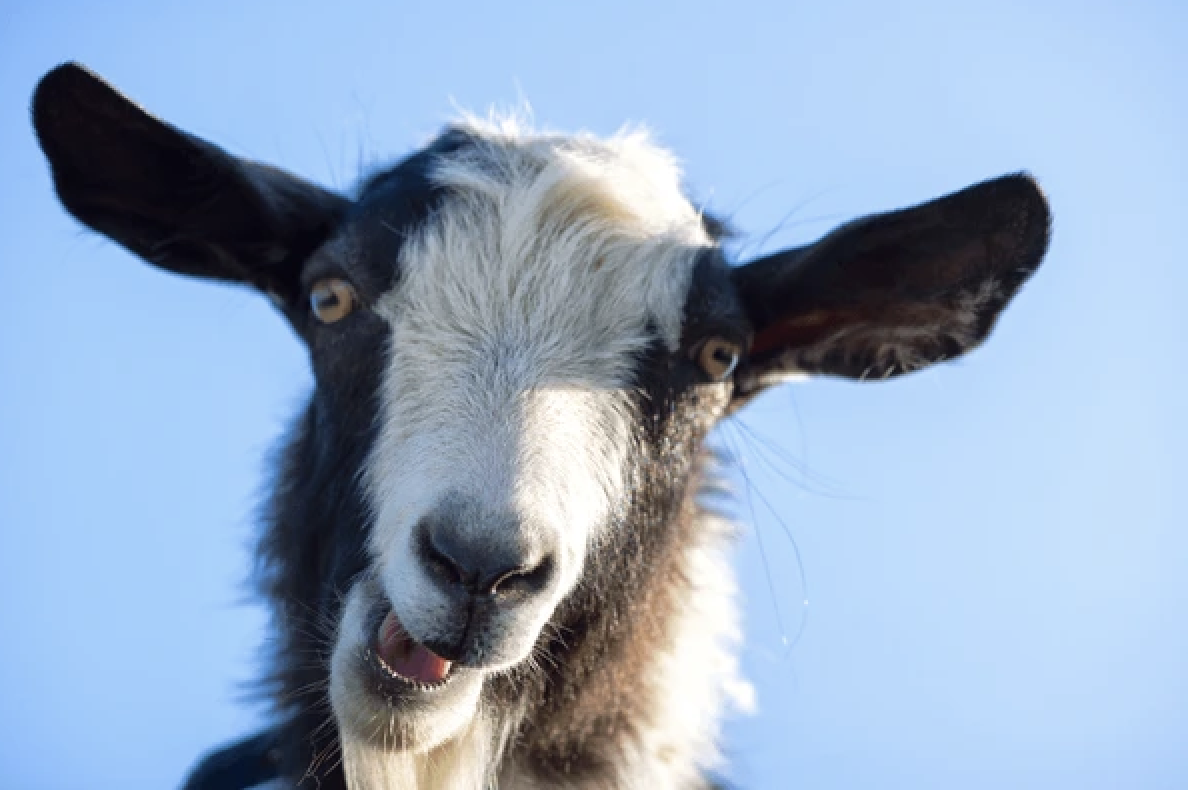
\includegraphics[width=0.35\textwidth]{images/goat.png}
	\end{figure}


\item {\bfseries\itshape I want cheesecake} Me too\dots
	\begin{figure}[H]
	\centering
	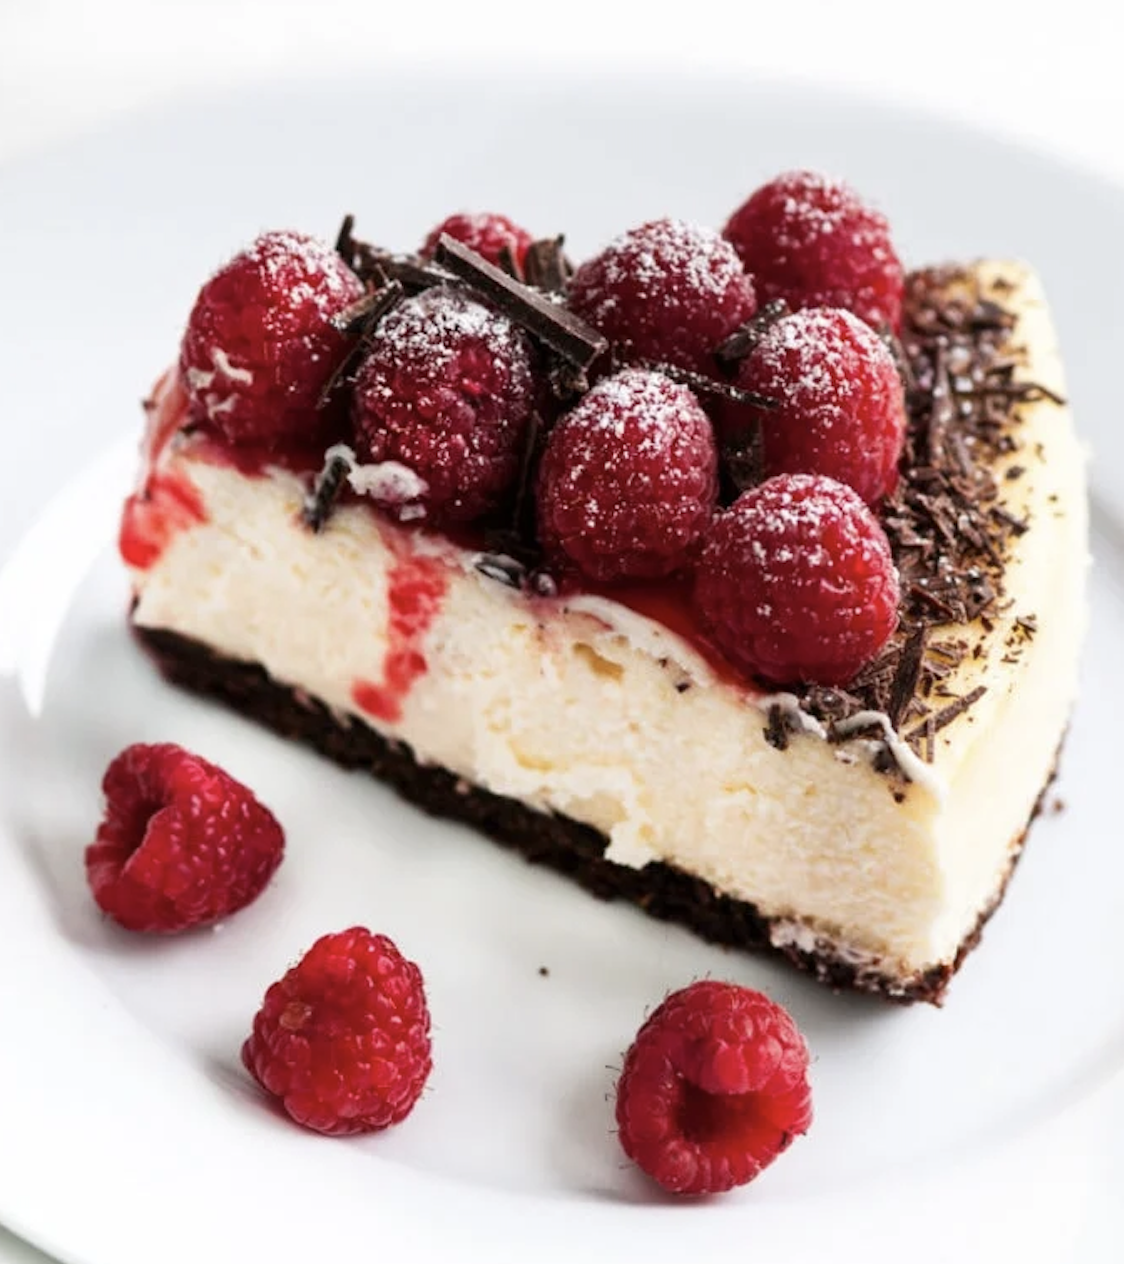
\includegraphics[width=0.35\textwidth]{images/cheesecake.png}
	\end{figure}

\item {\bfseries\itshape Do you actually read these? Draw a smiley on Monday on the board if you do.} I won't be blackmailed!

\item {\bfseries\itshape I'm watching Jujutsu Kaisen---it's awesome} I wouldn't go that far. It's okay. But don't say that in public, lest the fans come for you like the zombies in 28~Weeks Later. 

\item {\bfseries\itshape Do a Morgan Freeman impression} No. Now, I know what you want. What you're waiting for. That voice. The one folks say could make a grocery list sound like poetry. But that ain't what you'll find here. I won't pretend to be him. All I can do is speak plainly, in my own way. Some impressions are best left unsaid\dots and maybe that’s enough. 

\item {\bfseries\itshape How tf are spheres 2-dimensional? Please elaborate} `Dimension' is essentially how many variables you need to `track' the system. For instance, a line is 1-dimensional because you can keep track of it with one variable: if the line is $y= mx + b$, every point is of the form $(x, y)$ but $y= mx + b$ so that every point is of the form $(x, mx + b)$---only one variable $x$. Of course, we can imbed a line in two dimensions. Similarly, we live in a three dimensional world but there are two dimensional objects embedded in it. Give me a sphere of a certain radius, you only need 2 variables to keep track of where you are on it; hence, two dimensions. Think Earth. Big ole sphere. But give me your latitude and longitude and I know where you are.

\item {\bfseries\itshape If there are infinitely many numbers between 0 and 1 and between 1 and 2, why isn't the amount of numbers between 0 and 2 bigger but isn't it also infinite?} There are infinitely many numbers between 0 and 1, 1 and 2, and 0 and 2. And there are the same amount of numbers in all three of those. By counting you mean correspondence between `objects' and the numbers $\{1, 2, 3, \ldots, n \}$. In the infinite case, we just want a correspondence. Notice for each number in $[0, 1]$, I can get one and exactly one number in $[0, 2]$ by taking the number $x$ and doubling it. I can also go the other direction by cutting a number in half. Different numbers, sure. But the same number of numbers. Like counting $1, 2, 3, \ldots$ and $2, 4, 6, \ldots$. Different numbers. But clearly doubling/halving creates a correspondence between them. Hence, there are are just as many numbers in $\{1, 2, 3, \ldots \}$ as $\{2 , 4, 6, 8, \ldots \}$. There's a one-to-one correspondence between the numbers. Hence, the sets have the same `size.'
\end{itemize}

% 09/03, Wednesday: Continuity
\newpage
\section*{09/03, Wednesday: Continuity\label{09-03}}

\begin{itemize}
\item {\bfseries\itshape Class Rating:} 8.78/10

\item {\bfseries\itshape The Gateway video helped a great amount, thank you.} Thanks! Glad you found it helpful. Maybe I shouldn't say this, but it was actually kinda fun\dots

\item {\bfseries\itshape Do we need to show work for every step?} You do not need to show all your steps, especially for algebra. But what work needs to be shown depends on the problem. As a general rule of thumb, skipping algebra can be fine. Skipping Calculus is not fine. 

\item {\bfseries\itshape When is the exam?} All the exam dates are on the last page of the syllabus, on the back page of the Syllabus Quick Facts page, and they are also all in your Blackboard schedule. 

\item {\bfseries\itshape Are the tests in-person and do we have longer than 50~minutes?} They are all during lecture, in-person, and you only have the normal class 50~minutes. It's then very important to be on-time!

\item {\bfseries\itshape Will we cover squeeze theorem? We went over it in recitation} We did cover it in class---except one class where I needed 2--3 minutes more but mentioned to finish up the class by watching that section in one of the other classes lecture video. 

\item {\bfseries\itshape Does attendance in recitation affect grades?} Nope! There is a percentage displayed, but that percentage is not factored into the course average. 

\item {\bfseries\itshape What is the format of the exam?} There are a series of questions to answer. I'm not being flippant. I'm just not sure how to answer. Depending on what you meant, I may refuse to answer. I don't often reveal the number of questions, question formats, type of questions, etc. Looking at old exams you can see patterns, but the exam may not look like those. What you can feel rest assured about is that the exam will reflect the course material and be doable in the class time using the topics that we covered. I want you to learn Calculus, not learn how to do well on a specific type of test. 

\item {\bfseries\itshape I need help preparing for the exam} That's perfectly fine! I will be posting stuff about the exam that should cover this. 

\item {\bfseries\itshape Maybe explain problems like `Find $a, b$ so that $f(x)$ is continuous'} These are great problems to test your knowledge! It only uses the definition of continuity. Think, you know certainly things have to happen, i.e. certain limits have to equal certain other things. Once you compute these and write things out, all of a sudden, you have equations that need to be solved. Solving those equations gives you the $a, b$ you want!

\item {\bfseries\itshape Please draw more quick graphs that helps visualize a lot} I can whenever possible, but the early material doesn't lend itself well to it. 

\item {\bfseries\itshape I liked the interaction in class} I try to include it when possible, but we also have just so very much to cover. 

\item {\bfseries\itshape Is the exam multiple choice or only given questions? Or a mixture?} See the comment above about the exam. But I rarely ever include multiple choice or true/false, etc. That does not mean the exam cannot include them. 

\item {\bfseries\itshape Can we do more of these problems in class? More continuity?} Unfortunately, we are done with continuity. If you still need help with it, feel free to stop by for more discussion/help!

\item {\bfseries\itshape Not excited for note taking} A lot of people are. It really is a pretty even split on whether people like notes from packets or not. 

\item {\bfseries\itshape One of the easier lectures to understand} Glad it all made sense to you!

\item {\bfseries\itshape I liked this} I know! Isn't math awesome?!

\item {\bfseries\itshape Thanks for telling us what we need to know} No problem. When we have to short-change some topics time-wise like continuity, I think it's only fair game. 

\item {\bfseries\itshape I found the examples extremely helpful.} Now try the homework ones to make sure things clicked!

\item {\bfseries\itshape Just the overall way you teach is super helpful} I wasn't wearing overalls? 

\item {\bfseries\itshape I hated the anime discussion. I hate anime and will never watch it.} 
	\begin{figure}[H]
	\centering
	
\includegraphics[width=0.45\textwidth]{images/anime3.jpg}
	\end{figure}

\item {\bfseries\itshape Is Attack on Titan peak anime?} No\dots
	\begin{figure}[H]
	\centering
	
\includegraphics[width=0.45\textwidth]{images/anime4.jpg}
	\end{figure}

\newpage

\item {\bfseries\itshape ``Ah, dungeon food'' winged lion, Dungeon Meshi} I love Laois. I want him protected at all cost. He is everything to me. 
	\begin{figure}[H]
	\centering
	
\includegraphics[width=0.28\textwidth]{images/laois.jpg}
	
\includegraphics[width=0.43\textwidth]{images/laois2.jpeg}
	\end{figure}

\item {\bfseries\itshape You know Ball (Frieren)} 
	\begin{figure}[H]
	\centering
	
\includegraphics[width=0.45\textwidth]{images/frieren.png}
	\end{figure}

\item {\bfseries\itshape AOT is the best show and anime ever made, if you disagree you're a child} Ah yes, that's a true AOT fan for sure!
	\begin{figure}[H]
	\centering
	
\includegraphics[width=0.40\textwidth]{images/aot.jpeg}
	\end{figure}

\newpage

\item {\bfseries\itshape Inuyasha > Frieren} You didn't grow up with that! That's not even an anime from your generation! 
	\begin{figure}[H]
	\centering
	
\includegraphics[width=0.40\textwidth]{images/magic.png}
	\end{figure}

\item {\bfseries\itshape Favorite Frieren character?} All of them. If I had to pick one, why would I not choose Fern when she has the best line, ``I want to eat snacks.'' 
\end{itemize}

% 08/29, Friday: Limit Techniques
\newpage
\section*{08/29, Friday: Limit Techniques\label{08-29}}

\begin{itemize}
\item {\bfseries\itshape Class Rating:} 9.11/10

\item {\bfseries\itshape Where are the extra videos on Blackboard you said you would post that are really slow videos explaining everything?} They are in the corresponding lecture folder in the Lecture folder. 

\item {\bfseries\itshape Thank you for not making people feel dumb when they ask questions} Even if you felt dumb. You know you're not dumb. So, you should know that you can do this---even if you get confused, frustrated, or struggle. It's fine to struggle or be frustrated. What's important is that you push through and keep going. Learning to be okay with struggle/anxiety and still push through is a \textit{serious} skill that is worth learning and can get you far in college/life.

\item {\bfseries\itshape Why did we do a lab for the first lab class and then yesterday's class was all limit review?} I am not sure what you mean? Maybe you think one day is reserved for one and the other for the other. Tuesday/Thursday are for labs or recitations, but they do not have to fall on the same day or even each occur each week. But everything can be found in the course schedule. 

\item {\bfseries\itshape Where can we find extra practice problems for learned concepts?} Homeworks! \Winkey Although, remember there are problems also on my website and \textit{a lot, a lot} of extra problems in the `External Resource' folder on Blackboard.

\item {\bfseries\itshape When is the first quiz?} There are no quizzes in this course. 

\item {\bfseries\itshape Have you ever used Bobo Botn Eastsdc"} \dots what???

\item {\bfseries\itshape This was explained well!} Thanks! I would no try the homework then!

\item {\bfseries\itshape I suck at this} It's perfectly fine to struggle! We don't learn things at the same rate. It's about having the perseverance to keep going. Even if you improve only a little bit after a lot of time, then it's only a matter of time and effort until you're insanely good. It's not about where you start; it's about where you end. 

\item {\bfseries\itshape Today was an ah-ha day} Like a laughing day or it locked in day?

\item {\bfseries\itshape How can I apply Calculus to Physics or simulation context?} We will talk about applications, at least a little. But many applications require far more class time that we don't have or far more Calculus than just Calculus I. 

\item {\bfseries\itshape Thanks for a great first full week of classes. This has actually been my favorite class so far. Have a great weekend.} Thanks! Glad that you're enjoying it!

\item {\bfseries\itshape Do we get a study guide for the exam?} I will be posting an exam preparation guide. 

\item {\bfseries\itshape Are there any dropped check-ins?} No, but there is the possibility for a slight check-in curve at the end. 

\item {\bfseries\itshape Will we have a review day before the exam?} I only wish we had the lectures for that. We do get 1 or 2 in-lecture exam review---but for the later, harder exams. You will have an exam review in recitation though!

\item {\bfseries\itshape Do your research on LeBron Bymon James, aka King James} King James was a king of England. So, I think you're confused. 

\item {\bfseries\itshape Na, great lecture!} Thanks! I try!

\item {\bfseries\itshape Everything today clicked for me so very good} Great! I would then try the homework to see how well it actually all clicked. 

\item {\bfseries\itshape This was very cool! Examples were the best!} I'm glad you enjoyed it!

\item {\bfseries\itshape Can we get a full lesson recap before our exams, in-person or online?} I only wish we had the lectures for that. We do get 1 or 2 in-lecture exam review---but for the later, harder exams. You will have an exam review in recitation though!

\item {\bfseries\itshape Chipotle is not that good} 
	\begin{figure}[H]
	\centering
	
\includegraphics[width=0.40\textwidth]{images/wrong.jpeg}
	\end{figure}

\item {\bfseries\itshape The best selling sandwich in England is the the BLT which includes both a fruit and a vegetable} I pulled up this fact but the source is very sketchy. Moreover, I find it hard to believe that they eat that over cheese sandwiches---or anything else with even less flavour. 

\item {\bfseries\itshape You lack ball knowledge} Actually, I know \href{https://en.wikipedia.org/wiki/Ball\_(mathematics)}{a lot about balls}. One might say that I'm an expert on balls. \url{https://en.wikipedia.org/wiki/Ball\_(mathematics)}

\item {\bfseries\itshape Jalen hurts or Justen bulbert} I don't know who these people are\dots

\item {\bfseries\itshape I get within 10~km on Geoguesser} I actually get so close that I'm inside the house.
	\begin{figure}[H]
	\centering
	
\includegraphics[width=0.30\textwidth]{images/geoguesser.jpeg}
	\end{figure}

\item {\bfseries\itshape How many languages do you speak?} Not so many nowadays and it depends on what you mean by `speak'. At one point, to various degrees, English, Spanish, French, German, Italian, Portuguese, and Russian. 

\item {\bfseries\itshape Chipotle servings have gotten too small} I'm less concerned about the size than the price. You charge me a reasonable amount, I won't complain about the size. Size. Doesn't. Matter.

\item {\bfseries\itshape Chipotle is the best} But now so very expensive. 

\item {\bfseries\itshape Dap me up} 
	\begin{figure}[H]
	\centering
	
\includegraphics[width=0.30\textwidth]{images/dap.jpg}
	\end{figure}

\item {\bfseries\itshape Skyline is the best fast food! I'm from Cincinnati} I've never heard of it. But sorry to hear about Cincinnati\dots
	\begin{figure}[H]
	\centering
	
\includegraphics[width=0.30\textwidth]{images/burnt.png}
	\end{figure}
\end{itemize}

% 08/27, Wednesday: Limit Techniques
\newpage
\section*{08/27, Wednesday: Limit Techniques\label{08-27}}

\begin{itemize}
\item {\bfseries\itshape Class Rating:} 8.81

\item {\bfseries\itshape There are a lot of different ways to solve limits.} That's what makes them both great and terrible. They will take some practice, so start the homework early!

\item {\bfseries\itshape I don't know when to use each type of limit} That can be a tough thing! Knowing which `trick' to use takes practice until you start to see what time of limit it is. There are some rules of thumb: 1/0 is a thinking limit, rational functions at $\pm \infty$ are rational limits, root limits will tend to be conjugation tricks, etc. 

\item {\bfseries\itshape I am guessing 6.5/10 doesn't count for the Gateway?} No, sorry. It's a minimum of 7 points for a passing score. 

\item {\bfseries\itshape When is the second Gateway?} It's not till the end of September. The exam date you will take it is on the last page of the Syllabus or the back of the Syllabus Quick Facts. You can also open it in Blackboard to see when the exam and practice exam open. 

\item {\bfseries\itshape You Rick rolled me on Blackboard} I actually got the idea from someone else. A friend of mine in grad. school worked on a project joint with the Education department on farming student engagement through `social' interaction to improve their performance. It not only was kinda interesting---and I hate to admit it---it was actually kinda funny. You can \href{https://www.youtube.com/watch?v=dQw4w9WgXcQ}{read their article for free} if you wanted to check it out: \href{https://www.youtube.com/watch?v=dQw4w9WgXcQ}{https://artsandsciences.syracuse.edu/mathematics/news/graduate-student-reports-on-joint-education-project}

\item {\bfseries\itshape Math is hard} It's fine to find things hard. What matters is finding the perseverance to push through until you're able to figure it out. We may not all start at the same place or progress in the same way. But what matters is that we end in the same place. 

\item {\bfseries\itshape It was all understandable today!} Great! If you feel you've nearly gotten it, then try the homework! That's the best way to figure that out. 

\item {\bfseries\itshape I would appreciate more algebra explanation on cancelling numbers to `make it work' for $e$ limits} This would then be a great question for office hours or to stop by an SI session or to see your TA! 

\item {\bfseries\itshape Mask made it harder to hear} Sorry. Life is like that sometimes. But soon I shall be unmasked\dots which almost sounds like a threat. But it isn't. 

\item {\bfseries\itshape Feel better soon!} Thanks, I shall try!

\item {\bfseries\itshape You da man} I read 'dharmann' and was greatly confused. 

\item {\bfseries\itshape What do you enjoy about [?]} Because what you wrote is illegible. I shall make something up. I'm going to go with Thanksgiving. And obviously, the best answer is the mashed potatoes. 
	\begin{figure}[H]
	\centering
	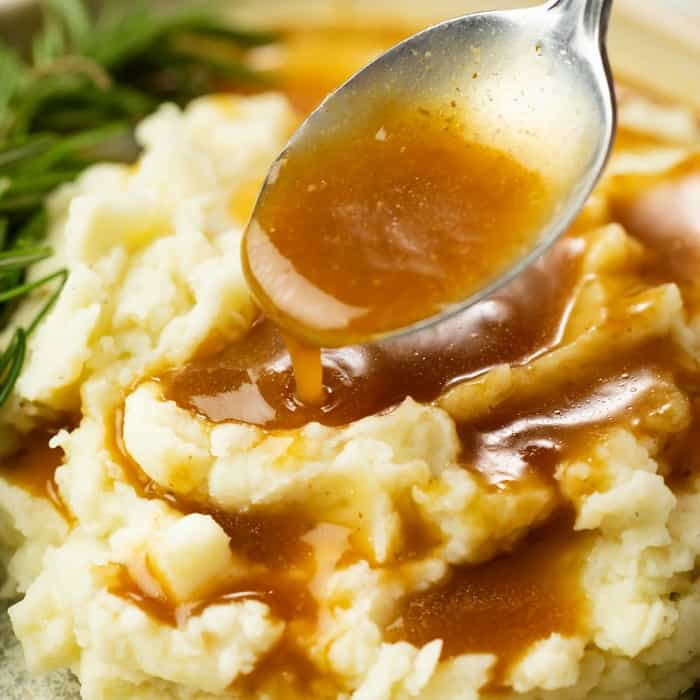
\includegraphics[width=0.2\textwidth]{images/potato.jpg}
	\end{figure}

\item {\bfseries\itshape Get well soon!} Thanks! If not, I will be forced to seek vengeance. 

\item {\bfseries\itshape Thank you for the Gateway video!} Anytime! It was kinda fun, not gonna lie.

\item {\bfseries\itshape Confused most of the time but it comes together in the end} That's all that matters---eventually getting it! If things don't eventually click, please, remember to stop by for help!

\item {\bfseries\itshape This wasn't as confusing and as complicated as the last class} Great! I am glad things are little by little making more sense! That's the goal!

\item {\bfseries\itshape Do you watch anime or only live TV?} I don't know anyone that watches live TV. Cable is dead. But yes, I watch anime. 
	\begin{figure}[H]
	\centering
	
\includegraphics[width=0.2\textwidth]{images/ablaze.jpg}
	\end{figure}

\item {\bfseries\itshape I like your `dumb' analogies} \dots if they were useful, wouldn't that make them smart analogies?

\item {\bfseries\itshape Python sucks} I know the labs may not be the most fun thing in the world, but Python as a programming language is super useful, super applicable, and super found everywhere! So, knowing even a tiny bit is not at all a bad things. Maybe view it that way?

\item {\bfseries\itshape Yooooooo} 
	\begin{figure}[H]
	\centering
	
\includegraphics[width=0.25\textwidth]{images/yoohoo.png}
	\end{figure}

\item {\bfseries\itshape You should try hockey, it's like polo with more fights and more missing teeth} Nope. No sports. My only interest would be for other reasons. 

\item {\bfseries\itshape Get well soon!} Thanks! I guess the only chance is to not and die. But I can't with so much TV yet to watch. 
	\begin{figure}[H]
	\centering
	
\includegraphics[width=0.2\textwidth]{images/murderbot.jpeg}
	\end{figure}

\item {\bfseries\itshape You remind me of a hyperactive Yorkie} \dots very daring of you to say so. Perhaps you have forgotten. 
	\begin{figure}[H]
	\centering
	
\includegraphics[width=0.4\textwidth]{images/skills.jpg}
	\end{figure}
\end{itemize}

% 08/25, Monday: Limit Techniques
\newpage
\section*{08/25, Monday: Limit Techniques\label{08-25}}

\begin{itemize}
\item {\bfseries\itshape Class Rating:} 8.63/10
\item {\bfseries\itshape Do we need a calculator for this class?} Nope! In fact, none is even allowed. 
	\begin{figure}[H]
	\centering
	
\includegraphics[width=0.2\textwidth]{images/calculator.jpg}
	\end{figure}

\item {\bfseries\itshape How do I know which homework correlates with each class period/lesson?} By the title, which should approximately correspond to the lecture titles. But you can always ask and I am happy to point it out!

\item {\bfseries\itshape Could you go over all the steps? Sometimes you skip steps} I try to balance this. I don't want to show so many that we take a lot of time and then don't cover things or see less problems. But I do not want to skip so much that I lose everyone. I try to show enough that I keep the vast majority of the room---though it may lose some folks. You can always go back in later and try to fill in the missing steps. Indeed, this is how you get better at the algebra!

\item {\bfseries\itshape Where can I practice limit problems?} Homeworks! Always start there. Beyond that, there are tons of extra problems broken down by topic in the `External Resources' folder on Blackboard. 

\item {\bfseries\itshape How do you remember and especially identify when we see certain problems?} That is the hard part---knowing which type of limit is which. There are some rules of thumb. However, this mostly comes down to experience. So, you need to do enough problems until you get a `feel' for it! 

\item {\bfseries\itshape If there were a campus shooting, where would we hide?} The general guidelines are run, hide, fight. Meaning, generally your first goal is to leave the area, not necessarily hide. This would then depend on the area---either towards center campus or across the bridge. In the classroom, that would be against the windows or chalkboard for hiding. And fight is always the last resort. You may always contact public safety if you want to know more of their guidelines for campus safety. 

\item {\bfseries\itshape You're my knight in shining armor} 
	\begin{figure}[H]
	\centering
	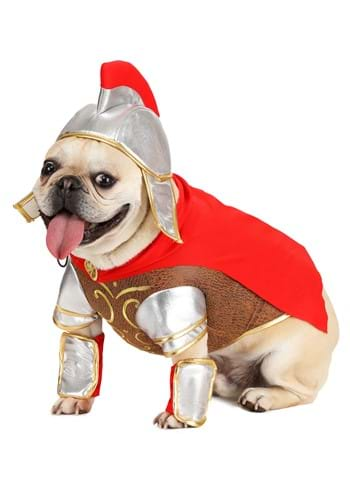
\includegraphics[width=0.15\textwidth]{images/pugcostume}
	\end{figure}

\item {\bfseries\itshape Are all the notes for the semester posted to Blackboard?} Indeed, they are! Also, the lecture videos are all posted---all broken down by lecture and labeled by the section.

\item {\bfseries\itshape Will points be taken off if we don't show the exact steps you show?} That depends on the steps. Generally, skipping some small algebra steps are fine. Skipping lots is bad. Skipping Calc steps is very bad. 

\item {\bfseries\itshape Should we know the unit circle?} Indeed! You should know all the trig functions value on the entire unit circle. There are resource videos on this in Blackboard to help!

\item {\bfseries\itshape How did you go from $\tfrac{\frac{1}{h + 5} - \frac{1}{5}}{h}$ to $\tfrac{\tfrac{5 - (h + 5)}{5(h + 5)}}{h}$?}
	\[
	\dfrac{\frac{1}{h + 5} - \frac{1}{5}}{h}= \dfrac{\frac{1}{h + 5} \cdot \frac{5}{5} - \frac{1}{5} \cdot \frac{h + 5}{h + 5}}{h}= \dfrac{\frac{5}{5(h + 5)} - \frac{h+5}{5(h + 5)}}{h}= \dfrac{\;\;\frac{5 - (h + 5)}{5(h + 5)}\;\;}{h}
	\]

\item {\bfseries\itshape Well explained!} Thanks! I tried!

\item {\bfseries\itshape Confused about the last limit with $e$} We will see more examples next class!

\item {\bfseries\itshape The examples are so helpful} There are plenty more in the homework \Winkey

\item {\bfseries\itshape Liked the werk method} Glad that you liked it!
	\begin{figure}[H]
	\centering
	
\includegraphics[width=0.25\textwidth]{images/werk.jpeg}
	\end{figure}

\item {\bfseries\itshape I would prefer to write my own notes} Never fear! We will only work from the packets for so long. After that, you will be expected to take your own notes.

\item {\bfseries\itshape Very helpful!} Thanks!

\item {\bfseries\itshape I'm looking forward to the semester} Thanks! Looking forward to working with you all!

\item {\bfseries\itshape I liked the lecture a lot I learned this concept in AP Calc and it was good way of teaching it. Also good emphasis on mental health} Thanks! Remember, the mental health sheet is on Blackboard so that you can always print more of them or click the links. Also, the resources are linked. 

\item {\bfseries\itshape People have been talking about homework being due but I don't see any due until September} I mentioned this in the syllabus video. All the homework is due two days before the exam. [So, students putting it off don't pull an all nighter right before an exam.] This schedule allows you to self pace or take breaks to focus on other courses or just a break. However, this means you have to keep track of pacing! I would suggest doing homeworks as soon as we finish the topics. 

\item {\bfseries\itshape Just gotta practice} Indeed! That is how you succeed in Mathematics. 

\item {\bfseries\itshape Please write a control of the problem and another that you work off of} I can try to remember. However, I do problems in-class essentially as I would like to see them done on exams. 

\item {\bfseries\itshape You contradicted some past statements} I did not. Which does that seem like?

\item {\bfseries\itshape You over-explained} I'm sorry. But I'd also rather go over than under!

\item {\bfseries\itshape Way better than my HS teacher!} Thanks!

\item {\bfseries\itshape Special limits was so friggin' tuff} It's fine to find things hard! Math can take some time to sit with stuff and practice. It's about the perseverance, not getting it right away. Of course, if things still don't sink in, please, ask questions, stop by for help, seek out the resources available to you! I want you to succeed!

\item {\bfseries\itshape I liked how you do an example and then we do a practice problem} I try to build in as much problem time as we can. But for some topics, that can be tough. 

\item {\bfseries\itshape You good baby girl}
	\begin{figure}[H]
	\centering
	
\includegraphics[width=0.20\textwidth]{images/blush.png}
	\end{figure}

\item {\bfseries\itshape You Rick rolled me :| } I was actually reading an article on Math Education and they had mentioned things like this as a method of student interaction. Overall, the article was really interesting and gave some nice insights into teaching and the student learning process. It's well worth checking out, \href{https://www.youtube.com/watch?v=dQw4w9WgXcQ}{http://mathworld.wolfram/math\_education/building-student-trust-and-engagement-in-the-classroom}

\item {\bfseries\itshape Still need help with conjugation!} You should hopefully do practice in recitation. There's also similar homework problems and also remember all the help resources available! 

\item {\bfseries\itshape What are different ways to memorize these?} Memorize what? The special limits? Not really that I can think of. But there's only 3!

\item {\bfseries\itshape Caleb, you talk very fast} I am sorry! It's who I am. Be comforted that most students do adjust to the cadence over time, just as one would with an accent. 

\item {\bfseries\itshape Favorite professional sports team?} I don't do sports. 

\item {\bfseries\itshape 67!} Easy, 36471110918188685288249859096605464427167635314049524593701628500- 267962436943872000000000000000.

\item {\bfseries\itshape Mandiballs} Mandibles?

\item {\bfseries\itshape $0 \cdot \infty= 1$???} Infinity is not a number, it has to come from a limiting process. So, depending on how the 0 and $\infty$ come about, yes, this is possible. We shall see this later in the course. Although, I believe I gave brief examples in lecture. 

\item {\bfseries\itshape You gotta watch a trailer for Weapons} Oh, there hasn't been a decent horror movie in years. Last one that was worth anything that I recall was The Witch. Although, Megan gave me a decent laugh. 

\item {\bfseries\itshape Recommended movies?} Oh, that really depends on what you're like and looking for. 

\item {\bfseries\itshape It's crazy how you kept track of every movie and TV show that you've ever watched, presumably since childhood} It's not as hard as you think. As of now, 2,986 movies and TV shows.

\item {\bfseries\itshape Least favorite food?} Liver.

\item {\bfseries\itshape You scare me} Now I know I'm not the best looking person, but to say that my looks are scary----how rude! But honestly, I don't judge and I'm here to help for as long as I have the time and you have the motivation to keep going!

\item {\bfseries\itshape I still think you look like Ian Hecox} We've covered this!
	\begin{figure}[H]
	\centering
	
\includegraphics[width=0.15\textwidth]{images/handsomesquidward.jpg}
	\end{figure}

\item {\bfseries\itshape Thank god for Project Runway} I've never actually seen it\dots

\item {\bfseries\itshape Are you into DND?} I've never played. Does not seem to be my thing. But I really like Baldur's Gate.
	\begin{figure}[H]
	\centering
	
\includegraphics[width=0.365\textwidth]{images/baldur.jpg}
	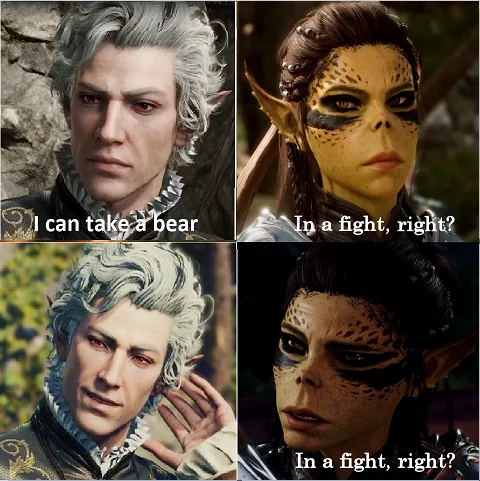
\includegraphics[width=0.25\textwidth]{images/baldur2.png}
	
\includegraphics[width=0.36\textwidth]{images/baldur3.png}
	\end{figure}

\item {\bfseries\itshape Why was 6 afraid of 7?} You're probably thinking because 7 ate (8) 9. But 6 has a greater fear after Fibonacci informed 6 that 5 ate (8) 13. 
	\begin{figure}[H]
	\centering
	
\includegraphics[width=0.15\textwidth]{images/handsomesquidward.jpg}
	\end{figure}

\item {\bfseries\itshape What's your favorite word in German?} Genau or perhaps uberlassen.
\end{itemize}

% 08/22, Friday: Limit Techniques
\newpage
\section*{08/22, Friday: Limit Techniques\label{08-22}}

\begin{itemize}
\item {\bfseries\itshape Class Rating:} 8.92/10

\item {\bfseries\itshape What's the point of the Python labs?} The department feels seeing some programming and `experiencing' the Calculus is important. Although, this (insofar as I am aware) comes from the School of Engineering. 

\item {\bfseries\itshape How do you plug in $\infty$ into a limit?} You don't! But you often do need to think about what happens when $x$ becomes infinitely large to compute some limits. Remember, $\infty$ is not a number. 

\item {\bfseries\itshape Will I need to know things like $\arctan$ for exams because I passed the gateway without it but I have never been taught it.} Though it likely won't show up often, you are expected to know the inverse trig function values. 

\item {\bfseries\itshape What is the best tool to use to brush up on my trig. values, inverse, etc. precalc stuff?} For trig, I think that I have everything you'd need on Blackboard. As for the algebra stuff, I'm not quite sure. Even Khan Academy or OrganicChemTutor might be sufficient for the course. 

\item {\bfseries\itshape What is the difference between DNE and undefined?} A limit does not exist if the right or left hand limit does not exist or they do not `align'. A function is undefined a value if it does not have a value there. 

\item {\bfseries\itshape What do you mean by you dropped your limits?} If you have a limit, say $\ds\lim_{x \to 0} \dfrac{\sin(3x)}{\tan(3x)}$, until you `plug-in' the limiting value---the final step---you must have that $\ds\lim_{x \to 0}$.

\item {\bfseries\itshape I liked that we had a chance to work out problems ourselves} We will try to build in time for that whenever possible. But depending on the topic, this might be more or less time. 

\item {\bfseries\itshape The examples were very helpful.} Thanks! I am glad that they clicked for you!

\item {\bfseries\itshape If you could do like a refresher on some of the way to get the equation before getting the answer} I'm happy to do a refresher on just about anything, but I'm not sure what you mean by getting the `equation'---we haven't seen any yet. So, I'm just unsure of what you're referring to. 

\item {\bfseries\itshape Being okay with being wrong makes me actually interested} It is always okay to be wrong, so long as one works towards not being wrong. Often, the first step in that direction is\dots well, being wrong! STEM courses/majors are hard. It's fine to be wrong or nervous or need to take some time to `get' things. It's not where you start, it's where you end. All it takes is the dedication to persevere. 

\item {\bfseries\itshape Great pacing today} Thanks!

\item {\bfseries\itshape Some parts went kinda fast} For the first day, for sure. But don't worry. We will (hopefully) have a decent pace as we move through limits. 

\item {\bfseries\itshape I feel like we went kind of quick over the asymptotes} Indeed, we did! Not all topics or facts are necessarily equally important in the course. You will notice that I will gloss over some points. This may be because, although it is nice to know, it is not terribly important. Such is the case with the asymptote information! 

\item {\bfseries\itshape Didn't know that $\sqrt{}$ can be in the denominator.} It certainly can! The square root of a number is just a number. There's nothing wrong with dividing a number by another---so long as that number isn't zero. The reason why $\tfrac{1}{\sqrt{2}}$ is written as $\tfrac{\sqrt{2}}{2}$ is because if one computed this by hand, for the former one would have to long divide 1 by $\sqrt{2}$---hard---while for the latter one just has to cut $\sqrt{2}$ in half---much easier. Of course, once calculators became cheap and prevalent, this became essentially pointless. In fact, in many cases, writing as the former is more useful for variety of reasons.  

\item {\bfseries\itshape It was nice to do some problems in class.} We will try to do as many problems as we can fit in class. Sometimes, this won't be much at all. Other times, it will be all that we do.

\item {\bfseries\itshape I would like to write my own notes.} Don't worry, we will eventually not be working from packets. So, you certainly will have the chance!

\item {\bfseries\itshape I think you answered questions really well and made it easy to understand} No problem! Always feel free to ask questions during lecture!

\item {\bfseries\itshape I both do and don't understand what I'm learning (not your fault though)} You may just need to sit with it a bit more. That's perfectly understandable! Remember, I post the lecture notes and video so you can always rewatch parts at your own pace. There's also lots of help options, including office hours, available to help you clear stuff up!

\item {\bfseries\itshape I am nervous, my last calc class was AB in junior year} No need to be nervous! You'll do great. There's lots of help and support for you at USC.

\item {\bfseries\itshape Great job answering questions} Thanks! I try!

\item {\bfseries\itshape The lab was confusing} Seeing Python will take some adjustment. But the department feels seeing some programming and `experiencing' the Calculus is important. 

\item {\bfseries\itshape Thanks for addressing common mistakes} No problem! I want you all to do well. 

\item {\bfseries\itshape Your vibe is not very boring so it makes it better to understand} Thanks! Although, I always assumed my vide was more anxious panda. 

\item {\bfseries\itshape You talk really fast but if I lock in I'm good.} I try to keep it in check. But over time, I assume ya'll will also adjust to my cadence. 

\item {\bfseries\itshape On the answer key on Blackboard, the example $\ds\lim_{b \to 0} \tfrac{(3 + b)^2 - 9}{b}= 9$ is wrong, it says 2 not 6.} Thanks! Who knows what I was doing at the time. Fixed!

\item {\bfseries\itshape Do you speak German? I heard you listening to an eBook when in your office} Yes or at least so-so. My German is not as good as it used to be. 

\item {\bfseries\itshape Day 1 of asking you to come to class barefoot} Absolutely not. What do you think this is, a hippie commune?! 

\item {\bfseries\itshape Caleb is a sigma goated beast} I don't know what that means. But I can only assume that means I'm like one of the following:
	\begin{figure}[H]
	\centering
	
\includegraphics[width=0.22\textwidth]{images/goat.jpg}
	
\includegraphics[width=0.22\textwidth]{images/baphomet.jpg}
	\end{figure}
I'm not sure which is worse\dots

\item {\bfseries\itshape Dr. McWhorter's celebrity lookalike is James C[G?]ordon} James Cordon? Hurtful. Besides, we've already covered my celebrity lookalike.
	\begin{figure}[H]
	\centering
	
\includegraphics[width=0.15\textwidth]{images/handsomesquidward.jpg}
	\end{figure}
\end{itemize}

% 08/20, Wednesday: Graphical Limits
\newpage
\section*{08/20, Wednesday: Graphical Limits\label{08-20}}

\begin{itemize}
\item {\bfseries\itshape Class Rating:} 8.69/10

\item {\bfseries\itshape How do you know if a function is `DNE' if there is a left and right limit?} We never say that a function is DNE, but we do say that a limit does not exist, i.e. DNE. This occurs when the left and right hand sides to not `approach' the same value. 

\item {\bfseries\itshape Sometimes when you pointed at the screen, I couldn't see and while I could figure it out, it added to the confusion at times} I will try to be better about remembering to use the highlight option. 

\item {\bfseries\itshape How is it sometimes DNE and $\infty$} It would depend on the limit. Some functions approach $\infty$ from both sides and hence the limit is $\infty$, similarly for $-\infty$. If the limit approaches different values---whether finite, $\infty$, or $-\infty$---from either side or infinitely `oscillates' then the limit does not exist (DNE). 

\item {\bfseries\itshape In the note directly under function behavior, does that say `examing'?} It says `examine'. 

\item {\bfseries\itshape Do you want us to raise our hands, or just blurt out the answer?} Yes\dots I mean, either is fine. 

\item {\bfseries\itshape Why do we write $x \to$ example and not use the variable $y$ as the answer?} While previous Math courses may have written $y$ instead of $f(x)$, we don't even need either in the case of others. For instance, if we had $\ds\lim_{x \to 1} (2x + 1)$, why would we need to introduce the notation $f(x)= 2x + 1$ or $y= 2x + 1$ and write $\ds\lim_{x \to 1} f(x)$ or $\ds\lim_{x \to 1} y$ when we could just write $\ds\lim_{x \to 1} (2x + 1)$?! And being that $\ds\lim_{x \to 1} (2x + 1)= 3$, we can just write that rather than using any notation with $y$. 

\item {\bfseries\itshape I think your communication is great, it is just hard to see the writing on board:} I will try to remember to write larger. While the packet print is small, you can also always print full sized versions using the PDFs on Blackboard if that helps!

\item {\bfseries\itshape Personally, I learn better with step by step explanations, will these be common in this class or would I benefit further from SI or outside sources?} It will depend on the topic and class. We only get so much time in lecture. Of course, if you need more detailed explanation, you can always feel free to stop by office hours for myself or the TA, stop by SI sessions, go to the Math Lab, tutoring, etc. All the help resources are linked on Blackboard!

\item {\bfseries\itshape Do you think you can go through one or two problem step by step before moving on to a new topic?} I can try to be slower when possible. But for today, there was no work/steps to be shown! In the case of graphical limits, one simply writes down the answer. It is all about knowing what a limit \textit{is}. 

\item {\bfseries\itshape Could you break down how to write answers to limits?} Thus far, we have only dealt with them graphically so there is no work to be shown and we only need write down the value! 

\item {\bfseries\itshape I've never taken a calculus course, so I'm unsure of what material to brush up on before this class.} I would say practice all your unit circle angles for all your trig functions---forwards and backwards, practice factoring and expanding polynomials, obtaining common denominators for rational functions, and review your power rules. There may be more, but remembering and being comfortable with all that gets you very far. 

\item {\bfseries\itshape Funny prof, made it understandable:} Well, glad someone thinks that I'm funny!

\item {\bfseries\itshape It was a little fast. You jumped into limits without explaining where the limit is and what it is.} I can totally understand how things may be a bit fast, especially for a first day. But that's exactly why I post the lecture notes and video so you can always rewatch part/all the lecture at your own pace. Know that explaining why we need limits and what a limit is was the first thing I did! Look at the notes/video at the bottom of the first page and the top of the second if you missed it. 

\item {\bfseries\itshape I wish the class was longer} Me too\dots me too\dots

\item {\bfseries\itshape I think I will enjoy this teaching style:} We shall see!

\item {\bfseries\itshape Thank you for not requiring a textbook. Thanks for being cool.} Well, Pearson is still required and costs about as much as any textbook. I'd like a cheaper/free option, but that's not so much up to me. 

\item {\bfseries\itshape I would have liked to write a little more:} We will only be working from the packets for the first little bit of the semester, and eventually you will need to take your own notes. 

\item {\bfseries\itshape The large packets are somewhat daunting} Don't worry! Those packets cover about the first 3-4 weeks of material. So, although it looks like a lot, we only cover a little bit of it each class. 

\item {\bfseries\itshape Caleb silly} No, Caleb tired. 

\item {\bfseries\itshape I loved the way you made it entertaining.} Isn't that why you're here?
	\begin{figure}[H]
	\centering
	
\includegraphics[width=0.40\textwidth]{images/entertained.jpg}
	\end{figure}

\item {\bfseries\itshape I really appreciate the resources you offered. I am a junior and have struggled with some stuff so I really appreciate it! Also you're super cool! :) } No problem! Remember, the mental health sheet is posted on Blackboard as well, so that you can always download more copies. Moreover, all the resources are also included individually and linked in Blackboard. 

\item {\bfseries\itshape You're very good at explaining stuff and the examples were great!} Thanks! I am glad you found them helpful! 

\item {\bfseries\itshape Has anyone ever told you that you remind them of Ian Hecox from Smosh?} I don't know who that is. But we all know who my real celebrity lookalike is\dots
	\begin{figure}[H]
	\centering
	
\includegraphics[width=0.15\textwidth]{images/handsomesquidward.jpg}
	\end{figure}

\item {\bfseries\itshape You are 1,000x better than my Pre-Calc professor \& looking forward to a great semester!} That's not fair! I deserve a fair shake to be terrible too! Give me a chance!

\item {\bfseries\itshape Is $1= 0.\overline{9}$} Yes! By $0.\overline{9}$ what is clearly meant is $0.9999\cdots$, which of course means $0.9 + 0.09 + 0.009 + \cdots$, which is\dots
	\[
	\sum_{n=1}^\infty 9 \left( \dfrac{1}{10} \right)^n= 9 \dfrac{\tfrac{1}{10}}{1 - \tfrac{1}{10}}= 9 \cdot \dfrac{\tfrac{1}{10}}{\tfrac{9}{10}}= 9 \cdot \dfrac{1}{9}= 1
	\]
where we have used the famous infamous geometric series sum formula. Alternatively, but less rigorously, we have\dots
	\begin{table}[!ht]
	\centering\small
	\begin{tabular}{lccc}
	& $10N$ & $=$ & $9.9999\overline{9}$ \\ 
	$-$ & $N$ & $=$ & $0.9999\overline{9}$ \\ \hline
	& $9N$ & $=$ & $9\phantom{.9999\overline{9}}$ \\
	& & $N= 1$ & 
	\end{tabular}
	\end{table}
\end{itemize}

\end{document}